\documentclass{standalone}
\usepackage{tikz}
\usepackage[]{tikzlings-koalas}
\usetikzlibrary{calc,patterns}
\newcommand{\footm}[1]{\mbox{\footnotesize{#1}}}
\begin{document}
	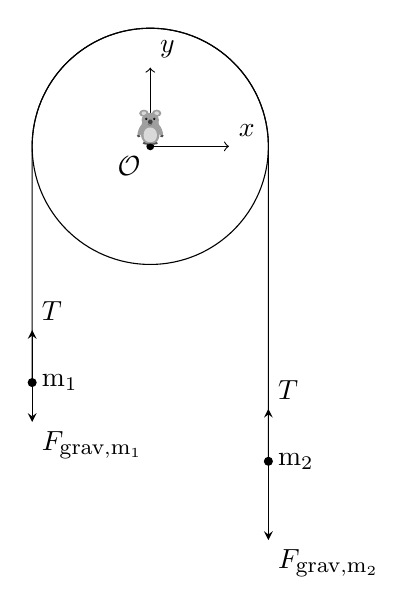
\begin{tikzpicture}
		\def\slength{3}
		\def\tlength{4}
		\def\pulleyradius{1.5}
		\def\ropethickness{.1}
		\def\gravitationalacceleration{.10}
		\def\smallmass{5}
		\def\bigmass{10}
		
		\coordinate (Pulley) at (0,0);
		\coordinate (Small) at (-\pulleyradius,-\slength);
		\coordinate (Big) at (\pulleyradius,-\tlength);
		
		\draw (Small) -- ++(0,\slength) arc[start angle = 180, end angle = 0, radius = \pulleyradius] -- ++ (0,-\tlength);
		
		\draw (Pulley) circle (\pulleyradius);
		\draw[fill] (Pulley) circle ({.01*\pulleyradius});
		
%		\draw (Small) -- ++({.07*\smallmass},0) -- ++({.02*\smallmass},{-.1*\smallmass}) -- ++({-2*.09*\smallmass},0) -- ++({.02*\smallmass},{.1*\smallmass}) -- ++({.07*\smallmass},0) -- cycle;
%		\draw (Big) -- ++({.07*\bigmass},0) -- ++({.02*\bigmass},{-.1*\bigmass}) -- ++({-2*.09*\bigmass},0) -- ++({.02*\bigmass},{.1*\bigmass}) -- ++({.07*\bigmass},0) -- cycle;
		
		\draw[fill] ({-\pulleyradius},{-\slength}) circle (.05) node[anchor = west] {\(\mbox{m}_1\)};
		\draw[fill] ({\pulleyradius},{-\tlength}) circle (.05) node[anchor = west] {\(\mbox{m}_2\)};
		
		\draw[-stealth] (-\pulleyradius,{-\slength}) -- ++(0,{-\gravitationalacceleration*\smallmass}) node[anchor = north west] {\(F_{\footm{grav},\footm{m}_1}\)};
		\draw[-stealth] (-\pulleyradius,-\slength) -- ++(0,{\smallmass*(\gravitationalacceleration*2*\bigmass/(\smallmass + \bigmass))}) node[anchor = south west] {\(T\)};
		\draw[-stealth] (\pulleyradius,{-\tlength}) -- ++(0,{-\gravitationalacceleration*\bigmass}) node[anchor = north west] {\(F_{\footm{grav},\footm{m}_2}\)};
		\draw[-stealth] (\pulleyradius,-\tlength) -- ++(0,{\smallmass*(\gravitationalacceleration*2*\bigmass/(\smallmass + \bigmass))}) node[anchor = south west] {\(T\)};
		
		\draw[-to] (Pulley) -- ++(0,1) node[anchor = south west] {\(y\)};
		\draw[-to] (Pulley) -- ++(1,0) node[anchor = south west] {\(x\)};
		\node[anchor = north east] at (Pulley) {\(\mathcal{O}\)};
		\fill (Pulley) circle (.05);
		\koala[scale = .2];
	\end{tikzpicture}
\end{document}
